Mis à part dans la partie consacrée à la documentation, nous présentons ici le reste du \textit{frontend} de l'\textit{API}.\\
Avant connexion, la page suivante se présente :
\begin{center}
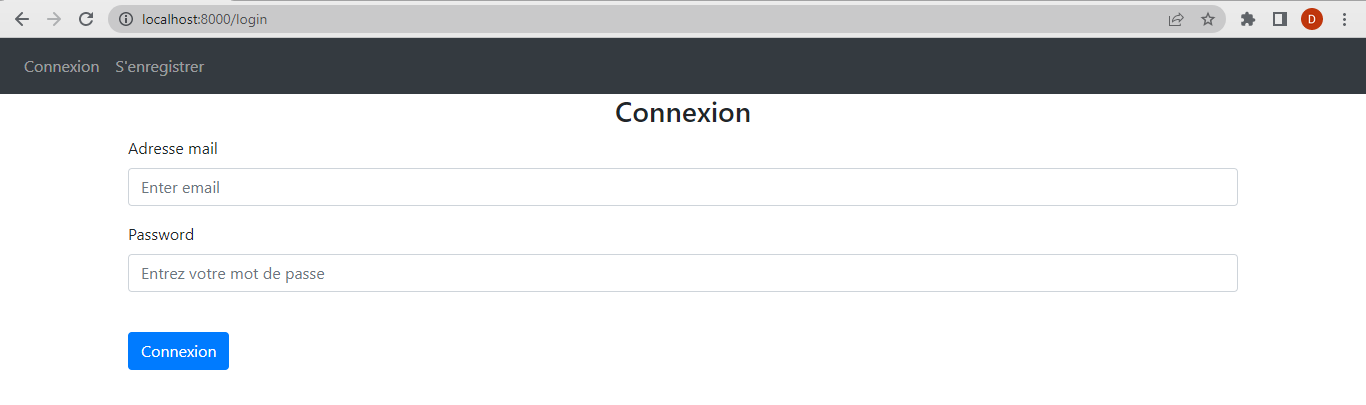
\includegraphics[width=15cm]{FrontAvantConnexion.PNG}
\end{center}
Après connexion, voici l'interface très succincte qui se présente :
\begin{center}
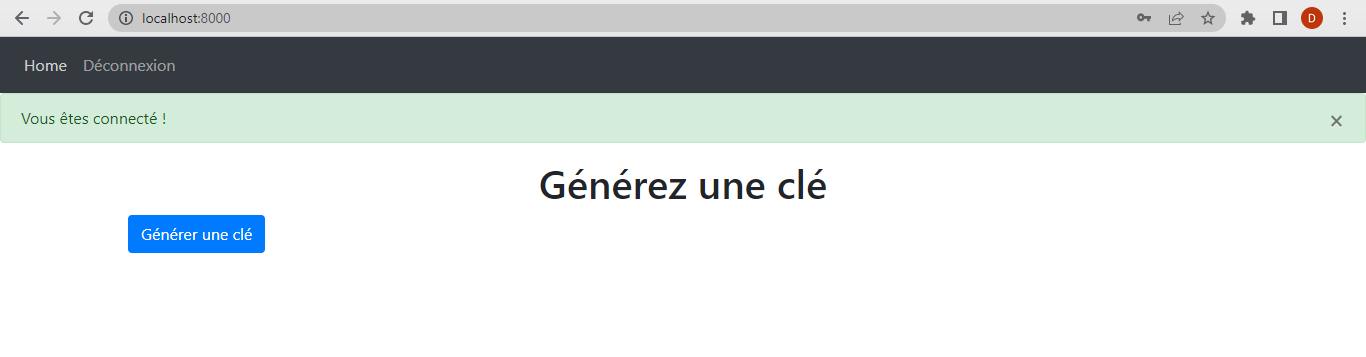
\includegraphics[width=15cm]{FrontApresConnexion.PNG}
\end{center}
Après génération de la clé, voici ce qui se présente :
\begin{center}
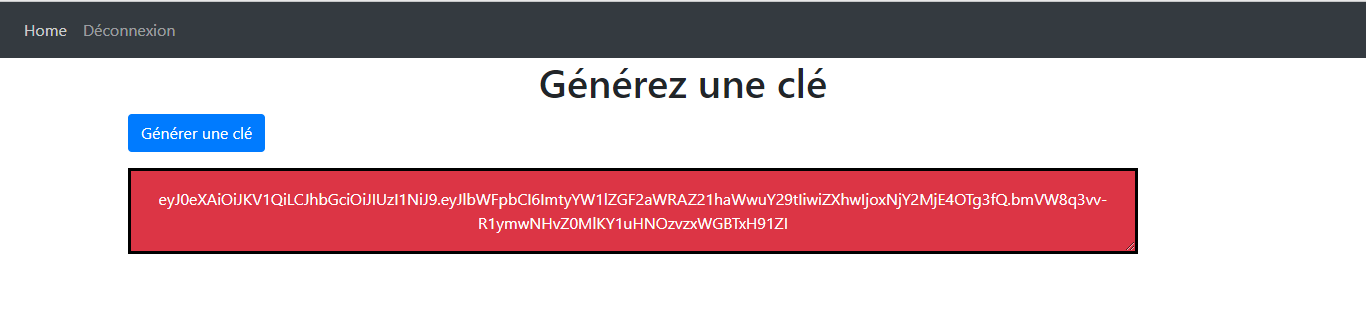
\includegraphics[width=15cm]{FrontApresGenCle.PNG}
\end{center}
Finalement, pour l'enregistrement, voici ce qui se présente :
\begin{center}
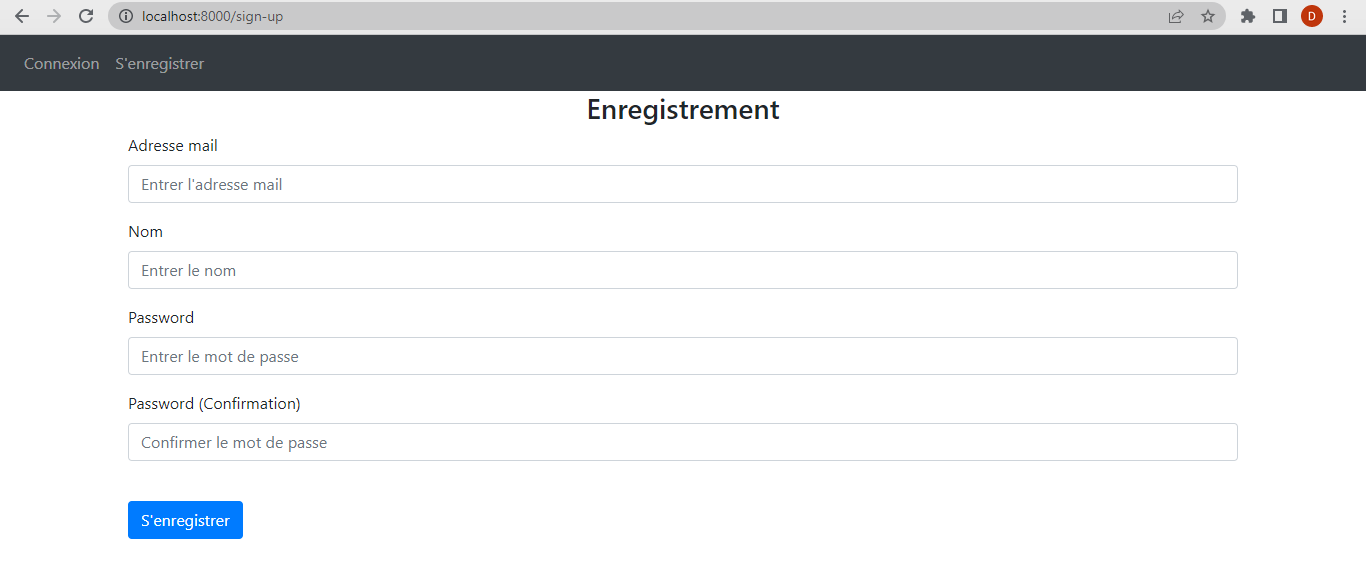
\includegraphics[width=15cm]{FrontEnregistrement.PNG}
\end{center}
Ceci est un ensemble d'interfaces très minimaliste mais on peut écrire quelques textes d'explication si nécessaire.